\chapter{Brief review of Fourier transforms}
\index{Fourier transform}

\subsection{Functional spaces}

That complex continuous waveforms or functions are comprised
of a number of harmonics seems to be an idea at least as old as the Pythagoreans.
In physical terms, Fourier analysis\cite{koerner,Howell,herman-fa}
attempts to decompose a function into its constituent harmonics, known as a frequency spectrum.
Thereby the goal is the expansion of periodic and aperiodic functions into sine and cosine functions.
Fourier's observation or conjecture is, informally speaking, that any   ``suitable''
function $f(x)$
can be expressed as a  possibly infinite  sum (i.e., linear combination), of sines
and cosines of the form
\begin{equation}
\begin{split}
f(x)
=
\sum_{k=-\infty}^\infty
\left[ A_k \cos (C k x) + B_k \sin (C k x)\right]\\
=
\left\{
\sum_{k=-\infty}^{-1} + \sum_{k=0}^\infty
\right\}
\left[ A_k \cos (C k x) + B_k \sin (C k x)\right]\\
=
\sum_{k=1}^{\infty}
\left[ A_{-k} \cos (-C k x) + B_{-k} \sin (-C k x)\right]  \qquad \qquad \\
+
\sum_{k=0}^\infty
\left[ A_k \cos (C k x) + B_k \sin (C k x)\right]\\
=
 A_0 +
\sum_{k=1}^{\infty}
\left[ \left( A_k+A_{-k} \right) \cos (C k x) + \left( B_k-B_{-k} \right) \sin (C k x)\right]
\\
=  \frac{a_0}{2} +
\sum_{k=1}^\infty
\left[ a_k  \cos (C k x) + b_k  \sin (C k x)\right]
,
\label{2012-m-ch-fourier_conjecture}
\end{split}
\end{equation}
with   $a_0=2 A_0$,
$a_k = A_k+ A_{-k}$,
and
$b_k = B_k- B_{-k}$.

Moreover, it is conjectured that any ``suitable''
function $f(x)$
can be expressed as a  possibly infinite  sum (i.e. linear combination), of exponentials; that is,
\begin{equation}
f(x)= \sum_{k=-\infty}^\infty
D_k e^{ikx}.
\label{2012-m-ch-fourier_conjecture1}
\end{equation}

More generally, it is conjectured that any ``suitable''
function $f(x)$
can be expressed as a  possibly infinite  sum (i.e. linear combination), of other (possibly orthonormal) functions $g_k( x)$; that is,
\begin{equation}
f(x)= \sum_{k=-\infty}^\infty
\gamma_k g_k(x).
\label{2012-m-ch-fourier_conjecturegen}
\end{equation}

The bigger picture can then be viewed in terms of
{\em functional (vector) spaces}: these are spanned by the elementary functions $g_k$, which serve as elements of a
{\em functional basis} of a possibly infinite-dimensional vector space.
\index{functional spaces}
Suppose, in further analogy to the set of all such functions ${\frak G}=\bigcup_k g_k(x)$
to the (Cartesian) standard basis, we can consider these elementary functions $g_k$ to be
{\em orthonormal} in the sense of a {\em generalized functional scalar product}
 [cf. also Section \ref{2012-m-sf-fs} on page \pageref{2012-m-sf-fs}; in particular
Equation (\ref{2011-m-ch-sfesp})]
\index{inner product}
\index{scalar product}
\begin{equation}
\langle   g_k \mid g_l\rangle
=
\int_{a}^b g_k(x)g_l(x)  \rho(x) dx =\delta_{kl}.
\label{2012-m-ch-sfesp1}
\end{equation}
For most of our purposes, $\rho (x)=1$.
One could arrange the coefficients $\gamma_k$ into a tuple (an ordered list of elements)
$(\gamma_1,\gamma_2, \ldots)$
and consider them as components or coordinates of a vector with respect to the
linear orthonormal functional basis ${\frak G}$.



\subsection{Fourier series}

Suppose that a function $f(x)$ is periodic -- that is, it repeats  its values in the interval $[-\frac{L}{2},\frac{L}{2}]$ --  with period $L$.
(Alternatively, the function may be only defined in this interval.)
A function $f(x)$
is {\em periodic}
\index{periodic function}
if there exist a period $L\in {\Bbb R}$ such that, for all $x$ in the domain of $f$,
\begin{equation}
f(L+x)=f(x).
\end{equation}

With certain ``mild'' conditions
-- that is, $f$ must be piecewise continuous, periodic with period $L$,  and (Riemann) integrable --
$f$ can be decomposed into a {\em Fourier series}
\index{Fourier series}
\begin{equation}
\begin{split}
f(x)={a_0\over2}+\sum_{k=1}^\infty
\left[a_k\cos\left(\frac{2\pi }{L}kx\right)+b_k\sin\left(\frac{2\pi }{L}kx\right)\right] \textrm{, with }\\
   a_k={2\over L}\int\limits_{-\frac{L}{2}}^\frac{L}{2}  f(x)\cos\left(\frac{2\pi }{L}kx\right) dx \textrm{ for } k \ge 0\\
   b_k={2\over L}\int\limits_{-\frac{L}{2}}^\frac{L}{2} f(x)\sin\left(\frac{2\pi }{L}kx\right) dx \textrm{ for } k > 0  .
\end{split}
\label{2012-m-ch-fs}
\end{equation}


{\color{OliveGreen}
\bproof

\marginnote{For proofs and additional information see \S~8.1 in \bibentry{Howell}.}
For a (heuristic) proof, consider the Fourier conjecture (\ref{2012-m-ch-fourier_conjecture}),
and compute the coefficients $A_k$, $B_k$, and $C$.

First, observe that we have assumed that $f$ is periodic with period $L$.
This should be reflected in the sine and cosine terms of   (\ref{2012-m-ch-fourier_conjecture}),
which themselves are periodic functions, repeating their values in the interval $[- \pi , \pi ]$; with period $2\pi$.
Thus in order to map the functional period of $f$ into the sines and cosines, we can ``stretch/shrink''
$L$ into $2\pi$; that is,
$C$ in Equation  (\ref{2012-m-ch-fourier_conjecture}) is identified with
\begin{equation}
C=\frac{2\pi}{L}.
\label{2012-m-ch-pfc1}
\end{equation}
Thus we obtain
\begin{equation}
f(x)= \sum_{k=-\infty}^\infty
\left[ A_k \cos \left(\frac{2\pi}{L} k x\right) + B_k \sin \left(\frac{2\pi}{L} k x\right)\right].
\label{2012-m-ch-pfc2}
\end{equation}

Now use the following properties:
(i)
for $k=0$, $\cos (0)=1$ and $\sin (0)=0$.
Thus, by comparing the coefficient $a_0$ in
(\ref{2012-m-ch-fs}) with $A_0$ in (\ref{2012-m-ch-fourier_conjecture})
we obtain  $A_0=\frac{a_0}{2}$.

(ii) Since $\cos (x)= \cos (-x)$ is an {\em even function} of $x$, we can rearrange the summation
by combining identical functions  $\cos (-\frac{2\pi}{L} k x) = \cos (\frac{2\pi}{L} k x) $,
thus obtaining $a_k = A_{-k}+A_k$ for $k>0$.

(iii) Since $\sin (x)= -\sin (-x)$ is an {\em odd function} of $x$, we can rearrange the summation
by combining identical functions  $\sin (-\frac{2\pi}{L} k x) =  -\sin (\frac{2\pi}{L} k x)$,
thus obtaining $b_k = -B_{-k}+B_k$ for $k>0$.

Having obtained the same form of the Fourier series of $f(x)$ as exposed in (\ref{2012-m-ch-fs}),
we now turn to the derivation of the coefficients $a_k$ and $b_k$.
$a_0$ can be derived by just considering the functional scalar product in
Equation (\ref{2012-m-ch-sfesp1})
of $f(x)$ with the constant identity function $g(x)=1$; that is,
\begin{equation}
\begin{split}
\langle   g  \mid f \rangle
=
\int_{-\frac{L}{2}}^\frac{L}{2} f(x)  dx \\
 =
\int_{-\frac{L}{2}}^\frac{L}{2} \left\{ \frac{a_0}{2}+\sum_{n=1}^\infty
\left[a_n\cos\left(\frac{2\pi}{L} n x\right)+b_n\sin\left(\frac{2\pi}{L} n x\right)\right]\right\}  dx  =
a_0\frac{L}{2}
,
\end{split}
\label{2012-m-ch-sfespnn}
\end{equation}
and hence
\begin{equation}
a_0 = \frac{2}{L} \int_{-\frac{L}{2}}^\frac{L}{2} f(x)  dx
\label{2012-m-ch-sfespnn2}
\end{equation}

In a similar manner, the other coefficients can be computed by considering
$\left\langle   \cos \left(\frac{2\pi }{L}kx\right)  \mid f(x) \right\rangle$
$\left\langle   \sin \left(\frac{2\pi }{L}kx\right)  \mid f(x) \right\rangle$
and exploiting the
{\em orthogonality relations for sines and cosines}
\index{orthogonality relations for sines and cosines}
\begin{equation}
\begin{split}
\int_{-\frac{L}{2}}^\frac{L}{2}
\sin\left(\frac{2\pi }{L}kx\right)
\cos\left(\frac{2\pi }{L}lx\right)
dx
=0,\\
\int_{-\frac{L}{2}}^\frac{L}{2}
\cos\left(\frac{2\pi }{L}kx\right)
\cos\left(\frac{2\pi }{L}lx\right)
dx
\\
=
\int_{-\frac{L}{2}}^\frac{L}{2}
\sin\left(\frac{2\pi }{L}kx\right)
\sin\left(\frac{2\pi }{L}lx\right)
dx
=\frac{L}{2}\delta_{kl}.
\end{split}
\label{2012-m-ch-orsc}
\end{equation}



\eproof
}

{
\color{blue}
\bexample
For the sake of an example, let us compute the  Fourier series of
$$
f(x)=\vert x\vert
=
\begin{cases}
 -x, & \textrm{ for }  -\pi \le x<0 ,\\
 +x, & \textrm{ for }  0\le x\le \pi  .
\end{cases}
$$

First observe that $L=2\pi$, and that
$f(x)=f(-x)$; that is, $f$ is an {\em even} function of $x$;
hence
$b_n=0$, and the coefficients $a_n$ can be obtained by considering only the integration
between $0$ and $\pi$.

For $n=0$,
$$a_0={1\over\pi}\int\limits_{-\pi}^\pi dxf(x)={2\over\pi}
\int\limits_0^\pi xdx=\pi.$$

For $n>0$,
\begin{eqnarray*}
   a_n&=&{1\over\pi}\int\limits_{-\pi}^\pi f(x)\cos(nx)dx=
         {2\over\pi}\int\limits_0^\pi x\cos(nx)dx=\\
      &=&{2\over\pi}\left[\left.{\sin(nx)\over n}x\right|_0^\pi-
         \int\limits_0^\pi{\sin(nx)\over n}dx\right]={2\over\pi}\left.
         {\cos(nx)\over n^2}\right|_0^\pi=\\
      &=&{2\over\pi}{\cos(n\pi)-1\over n^2}=-{4\over\pi n^2}\sin^2{n\pi\over2}=
         \left\{\begin{array}{cl}
              0&\mbox{for even $n$}\\
              \displaystyle-{4\over\pi n^2}&\mbox{for odd $n$}
              \end{array}\right.
\end{eqnarray*}
Thus,
\begin{eqnarray*}
    f(x)&=&{\pi\over2}-{4\over\pi}\left(\cos x+
               {\cos 3x\over9}+{\cos 5x\over 25}+\cdots\right)=\\
            &=&{\pi\over2}-{4\over\pi}\sum_{n=0}^\infty
               {\cos[(2n+1)x]\over(2n+1)^2}.
\end{eqnarray*}

\eexample
}

One could arrange the coefficients
$(a_0,a_1,b_1,a_2,b_2, \ldots)$
into a tuple (an ordered list of elements)
and consider them as components or coordinates of a vector spanned by the
linear independent sine and cosine functions which serve as a basis of an infinite
dimensional vector space.



\subsection{Exponential Fourier series}
\index{exponential Fourier series}




Suppose again that a function is periodic
with period $L$.
Then, under certain ``mild'' conditions
-- that is, $f$ must be piecewise continuous, periodic with period $L$,  and (Riemann) integrable --
$f$ can be decomposed  into an {\em exponential Fourier series}
\begin{equation}
\begin{split}
f(x)= \sum _{k=-\infty}^\infty c_k e^{ikx} \textrm{, with } \\
c_k=\frac{1}{L}\int_{-\frac{L}{2}}^{\frac{L}{2}} f(x') e^{-ikx'} dx'.
\end{split}
\label{2011-m-fa-e1fc}
\end{equation}

{\color{OliveGreen}
\bproof

The exponential form of the Fourier series
can be derived from the Fourier series (\ref{2012-m-ch-fs}) by
Euler's formula  (\ref{2012-m-ch-ca-ef}), in particular,
\index{Euler's formula}
$e^{ik\varphi} = \cos (k\varphi )+i \sin (k\varphi )$, and thus
$$
\cos (k\varphi ) =\frac{1}{2}\left(e^{ik\varphi}+e^{-ik\varphi}\right)
,\textrm{ as well as }
\sin (k\varphi ) =\frac{1}{2i}\left(e^{ik\varphi}-e^{-ik\varphi} \right)
.
$$
By comparing the coefficients of (\ref{2012-m-ch-fs}) with the coefficients of (\ref{2011-m-fa-e1fc}),
we obtain
\begin{equation}
\begin{split}
a_k= c_k+c_{-k} \textrm{ for } k \ge 0,\\
b_k= i(c_k-c_{-k})\textrm{ for } k > 0  ,\\
\end{split}
\label{2011-m-fa-e1fccc1}
\end{equation}
or
\begin{equation}
c_k=
\left\{
\begin{split}
\frac{1}{2}(a_k-ib_k) \textrm{ for } k > 0,\\
\frac{a_0}{2} \textrm{ for } k = 0,\\
\frac{1}{2}(a_{-k}+ib_{-k}) \textrm{ for } k < 0.
\end{split}
\right.
\label{2011-m-fa-e1fccc2}
\end{equation}

Eqs. (\ref{2011-m-fa-e1fc}) can be combined into
\begin{equation}
f(x)= \frac{1}{L}\sum _{\check{k}=-\infty}^\infty  \int_{-\frac{L}{2}}^\frac{L}{2} f(x') e^{-i{\check{k}(x'-x)}} dx'
.
\label{2011-m-eft1}
\end{equation}

\eproof
}




\subsection{Fourier transformation}

Suppose we define
$\Delta {k} = 2\pi /L$, or $1/L = \Delta {k} /2\pi$.
Then Equation (\ref{2011-m-eft1}) can be rewritten  as
\begin{equation}
f(x)= \frac{1}{2\pi}
\sum _{k=-\infty}^\infty  \int_{-\frac{L}{2}}^\frac{L}{2} f(x') e^{-i{{k}(x'-x)}} dx' \Delta {k}
.
\end{equation}
Now,
in the ``aperiodic'' limit $L\rightarrow \infty$ we obtain  the {\em Fourier transformation}
and the {\em Fourier inversion}
$
{\cal F}^{-1}[{\cal F} [f(x)]]=
{\cal F} [{\cal F}^{-1}[f(x)]]= f(x)
$
by
\index{Fourier transformation}
\index{Fourier inversion}
\begin{equation}
\begin{split}
f(x)= \frac{1}{2\pi}
 \int_{-\infty}^\infty   \int_{-\infty}^\infty f(x') e^{-i{{k}(x'-x)}} dx' d{k} \textrm{, whereby} \\
  {\cal F}^{-1}[\tilde{f}](x)=f(x)=  \alpha \int_{-\infty}^\infty \tilde{f}(k) e^{\pm i{kx}} dk \textrm{, and} \\
 {\cal F}[f](k)=\tilde{f}(k)=  \beta \int_{-\infty}^\infty  f(x') e^{\mp i{kx'}} dx'
.
\end{split}
\label{2011-m-efta}
\end{equation}
$ {\cal F}[f(x)]= \tilde{f}(k)$
is called the {\em Fourier transform}
\index{Fourier transform}
of $f(x)$.
%\marginnote{{\small http://home.comcast.net/$\sim$szemengtan/LinearSystems/fourier.pdf}}
{\em Per} convention, either one of the two sign pairs $+-$ or $-+$ must be chosen.
The factors $\alpha$ and $\beta$ must be chosen such that
\begin{equation}
 \alpha  \beta    = \frac{1}{2\pi};
\label{2011-m-efta1}
\end{equation}
that is, the factorization can be ``spread evenly among $\alpha$ and $\beta$,''
such that  $\alpha=\beta=1/\sqrt{2\pi}$, or ``unevenly,''
such as, for instance,
 $\alpha=1$ and $\beta=1/ 2\pi $,
or    $\alpha=1/ 2\pi $ and $\beta=1$.


Most generally, the Fourier transformations can be rewritten (change of integration constant),
 with arbitrary $A,B\in {\Bbb R}$,
as
\begin{equation}
\begin{split}
 {\cal F}^{-1}[\tilde{f}](x)=f(x)= B \int_{-\infty}^\infty \tilde{f}(k) e^{  iA{kx}} dk \textrm{, and} \\
 {\cal F}[f](k)=\tilde{f}(k)=  \frac{A}{2\pi B} \int_{-\infty}^\infty  f(x') e^{- iA{kx'}} dx'
.
\end{split}
\label{2011-m-efta1mg}
\end{equation}

The choice $A=2\pi $ and $B=1$ renders a  symmetric form of (\ref{2011-m-efta1mg}); more precisely,
\begin{equation}
\begin{split}
 {\cal F}^{-1}[\tilde{f}](x)=f(x)=   \int_{-\infty}^\infty \tilde{f}(k) e^{  2\pi i{kx}} dk \textrm{, and} \\
 {\cal F}[f](k)=\tilde{f}(k)=    \int_{-\infty}^\infty  f(x') e^{-  2\pi  i {kx'}} dx'
.
\end{split}
\label{2011-m-efta1mgAB1}
\end{equation}

{
\color{blue}
\bexample


For the sake of an example,
assume $A=2\pi $ and $B=1$  in Equation (\ref{2011-m-efta1mg}), therefore starting with (\ref{2011-m-efta1mgAB1}),
and consider the  Fourier transform of the  {\em Gaussian function}
\index{Gaussian function}
\begin{equation}
\varphi (x)= e^{-\pi x^2}   .
\label{2012-m-ch-fa-gaussian}
\end{equation}


As a hint, notice that
the analytic continuation of $e^{-t^2}$ is analytic in the region $0\le \vert {\rm Im}\,t\vert \le \sqrt{\pi }\vert k \vert$.
Furthermore, as will be shown in Eqs. (\ref{2012-m-ch-di-gi2}), the {\em Gaussian integral}
\index{Gaussian integral} is
\begin{equation}
\int_{-\infty}^\infty
 e^{-t^2} dt =\sqrt{\pi }  .
\end{equation}
With $A=2\pi $ and $B=1$  in Equation (\ref{2011-m-efta1mg}), the Fourier transform of the  Gaussian function is
\begin{equation}
\begin{split}
    {\cal F}[\varphi  ](k)=\widetilde{ \varphi} (k) =  \int\limits_{-\infty}^\infty
                 e^{-\pi  x^2}  e^{- 2\pi ikx} dx
\\
\textrm{[completing the exponent]}
              =
\int\limits_{-\infty}^\infty
                 e^{-{\pi  k^2}}e^{-\pi \left(x+{i}k\right)^2}   dx
\end{split}
\end{equation}
The variable transformation  $t=\sqrt{\pi} (x + {i}k) $
yields
$dt/ dx=\sqrt{\pi} $; thus $dx = dt/ \sqrt{\pi}$, and
\begin{equation}
   {\cal F}[\varphi  ](k)=\widetilde{ \varphi} (k)=\frac{ e^{-{\pi k^2}}}{\sqrt{\pi} }
                 \int\limits_{-\infty+i\sqrt{\pi} {k}}^{+\infty+i\sqrt{\pi} {k}}
                 e^{-t^2}  dt
\label{2012-m-ch-dergauin1}
\end{equation}

\begin{marginfigure}
\begin{center}
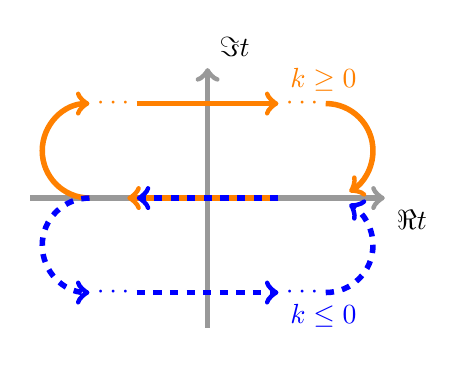
\begin{tikzpicture}  [scale=0.3]

\tikzstyle{every path}=[line width=2pt]

% Draw the axis

%\draw [color=black] (-3,0) -- (3,0);
%\draw [color=black] (0,-3) -- (0,3);
\draw[draw=gray!80,->] (0,-5) + (0,-0.5cm)  -- (0,5) -- +(0,0.5cm) node[above right] {$\Im t$};
\draw[draw=gray!80,->] (-7,0) +(-0.5cm,0) -- (7,0) -- +(0.5cm,0) node[below right] {$\Re t$};


\draw[orange,->] (-3,4) -- (3,4)  node[above right] {$k\ge 0$};
\draw[orange,->] (3,0) -- (-3.4,0) ;
\draw[color=blue,dashed,->] (-3,-4) -- (3,-4)  node[below right] {$k\le 0$};
\draw[color=blue,dashed,->] (3,0) -- (-3,0);

% Draw half circles

\draw [color=orange,->] (-5,0) arc [start angle=270,end angle=90,x radius=2cm, y radius=2cm];
\draw [color=orange,->] (5,4) arc [start angle=90,end angle=-60,x radius=2cm, y radius=2cm];
\draw [color=blue,dashed,->] (-5,0) arc [start angle=90,end angle=270,x radius=2cm, y radius=2cm];
\draw [color=blue,dashed,->] ( 5,-4) arc [start angle=-90,end angle=60,x radius=2cm, y radius=2cm];

\node[orange] at (-4,4) {$\cdots$};
\node[orange] at (4,4) {$\cdots$};
\node[blue] at (-4,-4) {$\cdots$};
\node[blue] at (4,-4) {$\cdots$};

\end{tikzpicture}
\end{center}
\caption{Integration paths to compute the  Fourier transform of the  Gaussian.}
\label{2011-m-ftgauss}
\end{marginfigure}
Let us rewrite the integration (\ref{2012-m-ch-dergauin1}) into the Gaussian integral by considering the closed paths
(depending on whether $k$ is positive or negative) depicted in Fig.~\ref{2011-m-ftgauss}.
whose ``left and right pieces vanish'' strongly as the real part goes to (minus) infinity.
Moreover,
by the Cauchy's integral theorem, Equation~(\ref{2018-m-ch-ca-cit}) on page~\pageref{2018-m-ch-ca-cit},
\index{Cauchy's integral theorem}
\begin{equation}
   \oint\limits_{\cal C} dt e^{-t^2}=\int\limits_{+\infty}^{-\infty}
  e^{-t^2} dt +\int\limits_{-\infty+{i\sqrt{\pi} }k}^{+\infty+{i\sqrt{\pi} }k}
   e^{-t^2} dt =0,
\end{equation}
because $e^{-t^2}$ is analytic in the region $0\le \vert {\rm Im}\,t\vert \le \sqrt{\pi }\vert k \vert$.
Thus, by substituting
\begin{equation}
 \int\limits_{-\infty+{i}\sqrt{\pi} k}^{+\infty+{i}\sqrt{\pi} k}
   e^{-t^2} dt =\int\limits_{-\infty}^{+\infty}e^{-t^2}  dt   ,
\end{equation}
in (\ref{2012-m-ch-dergauin1})
and  by insertion of the value
$\sqrt\pi$ for the {\em Gaussian integral},
as shown in  Equation (\ref{2012-m-ch-di-gi2}), we finally obtain
\begin{equation}
     {\cal F}[\varphi  ](k)=\widetilde{ \varphi} (k)=\frac{e^{-{\pi k^2 }}}{ \sqrt{\pi} }\underbrace{\int
   \limits_{-\infty}^{+\infty}e^{-t^2}dt}_{\mbox{$\sqrt\pi$}}=
   e^{-{\pi k^2}} .
\label{2012-m-ch-fa-gift}
\end{equation}

A similar calculation yields
\begin{equation}
     {\cal F}^{-1}[\widetilde{\varphi}  ](x)= \varphi (x)= e^{-{\pi x^2}} .
\label{2012-m-ch-fa-giftinverse}
\end{equation}
\eexample
}

Eqs.
(\ref{2012-m-ch-fa-gift})
and
(\ref{2012-m-ch-fa-giftinverse})
establish the fact that
the Gaussian function
$\varphi (x) = e^{-{\pi x^2}}$ defined in
(\ref{2012-m-ch-fa-gaussian})
is an {\em eigenfunction}
\index{eigenfunction}
\index{eigenvector}
of the Fourier transformations
${\cal F}$
and
${\cal F}^{-1}$ with associated eigenvalue $1$.
\marginnote{See Section~6.3 in \bibentry{strichartz}.}


With a slightly different definition the Gaussian function $f(x) = e^{-{x^2/2}}$ is also an eigenfunction of the operator
\begin{equation}
{\cal H} = - \frac{d^2}{d x^2} + x ^2
\label{2012-m-ch-fa-hphoe}
\end{equation}
corresponding to a harmonic oscillator.
The resulting eigenvalue equation is
\begin{equation}
\begin{split}
{\cal H} f(x) = \left(- \frac{d^2}{d x^2} +  x^2 \right) e^{-\frac{x^2}{2}}
=  -\frac{d }{d x }\left(-  x e^{-\frac{x^2}{2}} \right) +  x^2 e^{-\frac{x^2}{2}}  \\
=  e^{-\frac{x^2}{2}} -  x^2 e^{-\frac{x^2}{2}}  +  x^2 e^{-\frac{x^2}{2}}
= e^{-\frac{x^2}{2}}
=  f(x);
\label{2012-m-ch-fa-hphoeee}
\end{split}
\end{equation}
with eigenvalue $1$.
\if01
Let us introduce the
{\em creation}
and
{\em annihilation}
opertors
\index{creation opertors}
\index{annihilation opertors}
${\cal A}^\dagger =  \frac{d}{d x} -  x$
and
${\cal A}  =  - \frac{d}{d x} -  x$,
respectively.
Then,
${\cal A}^\dagger {\cal A}= {\cal H} -1$ and
${\cal A} {\cal A}^\dagger = {\cal H} +1$,
or
${\cal A}{\cal A}^\dagger {\cal A}= {\cal A}{\cal H} -{\cal A}$ and
${\cal A} {\cal A}^\dagger {\cal A}= {\cal H}{\cal A} +{\cal A}$,
and thus
$ {\cal A}{\cal H} -{\cal A} - {\cal H}{\cal A} - {\cal A} = 0$,
hence
$ [{\cal A},{\cal H}] = 2{\cal A}$.
\fi

Instead of going too much into the details here, it may suffice to say
that the
{\em Hermite functions}
\index{Hermite functions}
\begin{equation}
h_n(x) =\pi^{-1/4}(2^n n!)^{-1/2}\left(  \frac{d}{dx} -x\right)^n e^{-{x^2/2}}
= \pi^{-1/4}(2^n n!)^{-1/2} H_n(x) e^{-{x^2/2}}
\end{equation}
are all eigenfunctions of the Fourier transform with the eigenvalue $i^n \sqrt{2\pi }$.
The polynomial $H_n(x)$ of degree $n$ is called {\em Hermite polynomial}. \index{Hermite polynomial}
Hermite functions form a complete system, so that any function $g$ (with $\int \vert g (x) \vert^2 dx <\infty$) has a
{\em Hermite expansion}
\index{Hermite expansion}
\begin{equation}
g(x) = \sum_{k=0}^\infty \langle g , h_n\rangle h_n(x)
.
\end{equation}
This is an example of an
{\em eigenfunction expansion}.
\index{eigenfunction expansion}

\begin{center}
{\color{lightgray}   \Huge
\aldine
 %\decofourright \decofourleft
%\aldine X \decoone c \floweroneright
% \aldineleft ] \decosix g \leafleft
% \aldineright Y \decothreeleft f \leafNE
% \aldinesmall Z \decothreeright h \leafright
% \decofourleft a \decotwo d \starredbullet
% \decofourright b \floweroneleft
}
\end{center}
